\subsection{}
\index{Feshbach Resonance!Narrow}
One key ideas to hide all detail in high-energy (not clear yet) into some constant by renormalization.  All coupling are short-range (within potential range $r_{c}$), and we should hide it.  On the other hand, the detuning $\delta=E^{0}-\eta$ is not necessarily in this high-energy region for narrow resonance as it might smaller than Fermi energy.  In \eef{eq:20100915:tu}, detuning $\delta=E^{0}-\eta$ can get so large in part of fermi sea that $\tilde{U}$ becomes small.  We need to figure out a way to renormalize out the k-denpendence in $U_{\vk\vk'}$ and $Y_{\vk\vk'}$ but keep detuning around.  

\eef{eq:20100915:gap} is very similar to two-body \sch equation in zero energy.  However, the narrow resonance is probably more relevant with two-body \sch equation in finite energy.  How to bring it in?

\subsection{Chemical potential}
\emph{Chemical potential is determined in different ways between narrow or broad resonance.  }In broad case, it is determined mostly by open-channel \eef{eq:20100915:gapa}; in narrow case, chemical potential is determined by close-channel, where the close-channel bound-state level sits relative to Fermi sea.  In the extreme narrow case (without open-channel interaction as \cite{GurarieNarrow}), the level is exactly where chemical potential sits, cutting Fermi sea, depleting everything above in open-channel and putting them into close-channel.   

By correcting all equations in previous few sections and put the chemical potential $\mu$ in the proper position, we can see the narrow/broad resonance even in the four species case.  In Eq. (\ref{eq:20100915:t0}-\ref{eq:20100915:tk}), there are two many-body effects: $\sqrt{1-4G_{\vk}^{2}}$ from three-species Pauli exclusion; chemical potential in detuning term $E^{0}-\eta+\mu$, which is common in either three or four-species case.  And the later reduces to $\mu=0$ \footnote{In BEC side, $\mu<0$ and is controlled by mostly two-body attraction.  But that is not proper for real two-body limit, which should be $\mu=0$.}in zero-density which is two-body case. 
\begin{figure}[hhtb]
	\centering
		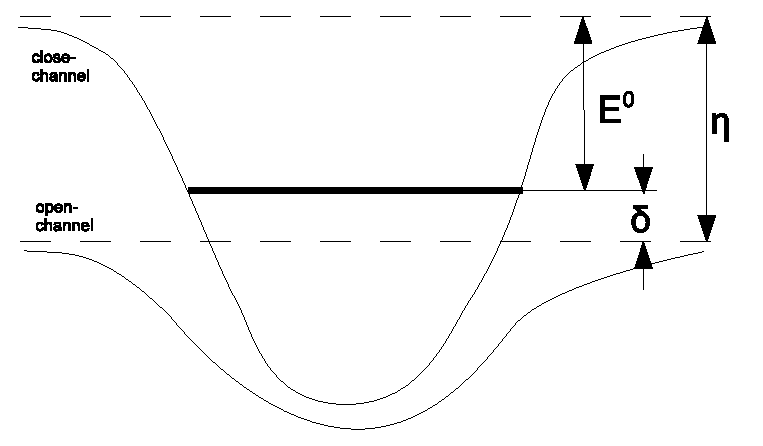
\includegraphics[width=.50\textwidth]{image/FeshbachPotential}
	\caption{Feshbach Resonance Potential\label{fig:FeshbachPotential}}	
\end{figure}

Imaging we start fairly far away from resonance (BCS side, $\delta=\eta-E^{0}>0$), and increase the density, in the beginning, $\mu$ is negligible, and inter-channel coupling term $\frac{Y_{\vk\vk''}Y_{\vk''\vk'}}{2(E^{0}-\eta+\mu)} $ is small; as $\mu$  increases, $-(\delta-\mu)$ gets closer and closer to zero, and this terms increases until the part of the Fermi sea gets into resonance.  





\subsection{Renormalization of gap equation}
There are more than one options to renormalize gap equation \eef{eq:20100915:onechannel}.  The part that needs to be renormalized out is  high energy summation of $\sqrt{\frac{(1-4G_{\vk'}^{2})}{{(\xi^{ab}_{\vk}+  G_{\vk}^2\eta)^{2}+\Delta_{\vk}^{2}}}}$, it approaches $\nth{\epsilon_{\vk}}$ in high energy.  Several sightly different physical quantities have the summation of the same high energy limit.  
\begin{enumerate}
\item The process used in Eq. (\ref{eq:20100915:t0}-\ref{eq:20100915:tk}).  This leads to the zero energy T-matrix of reduced DoS with factor $\sqrt{(1-4G_{\vk'}^{2})}$, with chemical potential in the detuning.  
\begin{equation}\tag{\ref{eq:20100915:renormGap}}
\nth{\tilde{t_{0}}(\mu)}=\sum_{\vk}\sqrt{(1-4G_{\vk}^{2})}
\br{\nth{\epsilon_{\vk}}-\nth{\sqrt{{(\xi^{ab}_{\vk}+  G_{\vk}^2\eta)^{2}+\Delta_{\vk}^{2}}}}}
\end{equation}
\begin{gather}
\tilde{t_{0}}(\mu)=\br{1-\tilde{U}\tilde{ K}}^{-1}\tilde{U}\tag{\ref{eq:20100915:t0}}\\
\tilde{U}_{\vk\vk'}=\nth{2} \br{U_{\vk\vk'}+\frac{Y_{\vk\vk''}Y_{\vk''\vk'}}{2(E^{0}-\eta+\mu)}}\tag{\ref{eq:20100915:tu}}\\
\tilde{K}=\frac{\sqrt{1-4G_{\vk}^{2}}}{\epsilon_{\vk}}\delta_{\vk\vk'}\tag{\ref{eq:20100915:tk}}
\end{gather}
\item We can also notice that $G_{\vk}\rightarrow0$ at high energy.  So we can simply takes the normal zero-energy T-matrix with detuning related to chemical potential.  
\begin{equation}\label{eq:20101004:renormGap1}
\nth{{t_{0}}(\mu)}=\sum_{\vk}
\br{\nth{\epsilon_{\vk}}-\frac{\sqrt{(1-4G_{\vk}^{2})}}{\sqrt{{(\xi^{ab}_{\vk}+  G_{\vk}^2\eta)^{2}+\Delta_{\vk}^{2}}}}}
\end{equation} 
\begin{gather}
{t_{0}}(\mu)=\br{1-\tilde{U}\tilde{ K}}^{-1}\tilde{U}\label{eq:20101004:t01}\\
\tilde{U}_{\vk\vk'}=\nth{2} \br{U_{\vk\vk'}+\frac{Y_{\vk\vk''}Y_{\vk''\vk'}}{2(E^{0}-\eta+\mu)}}\label{eq:20101004:tu1}\\
{K}=\nth{\epsilon_{\vk}}\delta_{\vk\vk'}\label{eq:20101004:tk1}
\end{gather}
Here Eqs. (\ref{eq:20101004:t01}-\ref{eq:20101004:tk1}) follows the same two-body formula for zero-energy T-matrix element.  However, the detuning is shifted by a many-body quantity $\mu$ that should be determined by solving gap equation with numberequation.    

\item  Alternatively, we notice that $\xi_{\vk}=\epsilon_{\vk}-\mu$, high energy limit can also be written as 
$\nth{\epsilon_{\vk}-\mu}$.  This leads to the T-matrix at energy $\mu$, the same detuning as before.  
\begin{equation}\label{eq:20101004:renormGap2}
\nth{{t_{\mu}}(\mu)}=\sum_{\vk'}
\br{\nth{\epsilon_{\vk'}-\mu}-\frac{\sqrt{(1-4G_{\vk'}^{2})}}{\sqrt{{(\xi^{ab}_{\vk}+  G_{\vk}^2\eta)^{2}+\Delta_{\vk}^{2}}}}}
\end{equation} 
\begin{gather}
{t_{\mu}}(\mu)=\br{1-\tilde{U}\tilde{ K}}^{-1}\tilde{U}\label{eq:20101004:t02}\\
\tilde{U}_{\vk\vk'}=\nth{2} \br{U_{\vk\vk'}+\frac{Y_{\vk\vk''}Y_{\vk''\vk'}}{2(E^{0}-\eta+\mu)}}\label{eq:20101004:tu2}\\
{K}=\nth{\epsilon_{\vk}-\mu}\delta_{\vk\vk'}\label{eq:20101004:tk2}
\end{gather}
The advantage of this is that introduce the effective range $r_{0}$ for finite energy T-matrix. 
\end{enumerate}

\subsection{Pauli exclusion factor  $\sqrt{(1-4G_{\vk'}^{2})}$ }
It seems that numerous Gap equations above has the Pauli-exclusion factor $\sqrt{(1-4G_{\vk'}^{2})}$.  Generally, 
\begin{equation}
G_{k=0}^{2}\sim{\frac{N_{close}}{N_{0}}\frac{r_{close}^{3}}{a_{0}^{3}}}
\end{equation}
where $r_{close}$ is close-channel molecule size, $N_{0}$ is the total number of fermions, $N_{close}$ is the number in close-channel, $a_{0}$ is the average particle distance.  This quantity is related the detail of close-channel bound-state.  We should relate it to some experimental available quantities.  In the above expression, factor $r_{close}^{3}/a_{0}^{3}$ relates to the two-body physics, while $N_{close}/N_{0}$ relates to many-body physics which probably needs to be solved consistently with the many-body equation .  

\subsection{More on chemical potential shift for detuning}
Let us image a sweep of $\delta$ from BCS end.  At the very BCS end, $\delta$ is positive and large than $\mu\approx{}E_{F}$ (Fig. \ref{fig:narrowFR:aboveSea}). Resonant term in interaction is relatively small and close-channel weight is small too.  We are very well in the  weak-attraction (slightly enhanced by resonance) BCS-like state in open-channel.  However, the detuning is shifted by $\mu\approx{}E_{F}$, so the resonance is reached earlier, and the larger the density, the earlier it does.  

As the detuning gets close to Fermi surface, chemical potential decreases from $E_{F}$. For narrow resonance, $E_{F}$ is large than the resonance energy scale.  The resonance reaches probably before detuning reaches Fermi surface.  If we ignore the shift due to open-channel intra-channel coupling for the moment, the resonance is very close at the point where $\delta=E_{F}$.  After $\delta$ drops into Fermi sea (Fig. \ref{fig:narrowFR:inSea}), chemical potential $\mu$ tracks the close-channel bound-state closely and the denominator of resonant term $-(\delta-\mu)$ keeps very small, and in some sense, the Feshbarch resonance is enhanced by the many-body  physics.  Open-channel still has energy advantages below $\mu$, so both channels are important.  

After $\delta$ drops below zero (Fig. \ref{fig:narrowFR:belowSea}), chemical potential still tracks $\delta$, but now most weight is in close-channel and the bound-state is mostly made of close-channel.  

\subsection{Number equation}
For number equation \eef{eq:20100909:number}, more approximation can be made in Feshbach resonance.  Close-channel component $G_{k}$ is much extended in k-space due to the tight-binding, and $F_{k}$ is significant up to the order of Fermi energy $E_{F}$.  It seems OK to assume that most weight of close-channel lies beyond $E_{F}$, so when $\epsilon_{k}\gg{E_{F}}$, the integrand becomes simply $G_{k}^{2}$, the summation gives $N_{close}$.  Therefore we have 
\begin{equation}\label{eq:20100909:number}
N_{open}=\sum_{\vk}{}^{'}\frac{1}{2} \left(1-\sgn_{k}\sqrt{1-4 F_{\vk}^2-4 G_{\vk}^2}\right)-G_{\vk}^{2}
\end{equation} 
Here the summation only goes up to the order of $E_{F}$